\subsection{Red de Centro Comercial}

En este caso la captura se llevó a cabo en una red no controlada, en el shopping Galerías Pacífico, durante aproximadamente 10 minutos.
Debido a que la red no está controlada por nosotros, no conocemos la naturaleza de los equipos que intercambian infomración en la misma, pero conjeturamos que la mayoría son teléfonos celulares.

\FloatBarrier

\subsubsection{Paquetes capturados e información}

Los resultados del experimento para determinar protocolos importantes para la fuente $S$ se resumen en los siguientes gráficos.

\begin{figure}[ht!]
  \centering
  \begin{minipage}[b]{0.48\textwidth}
    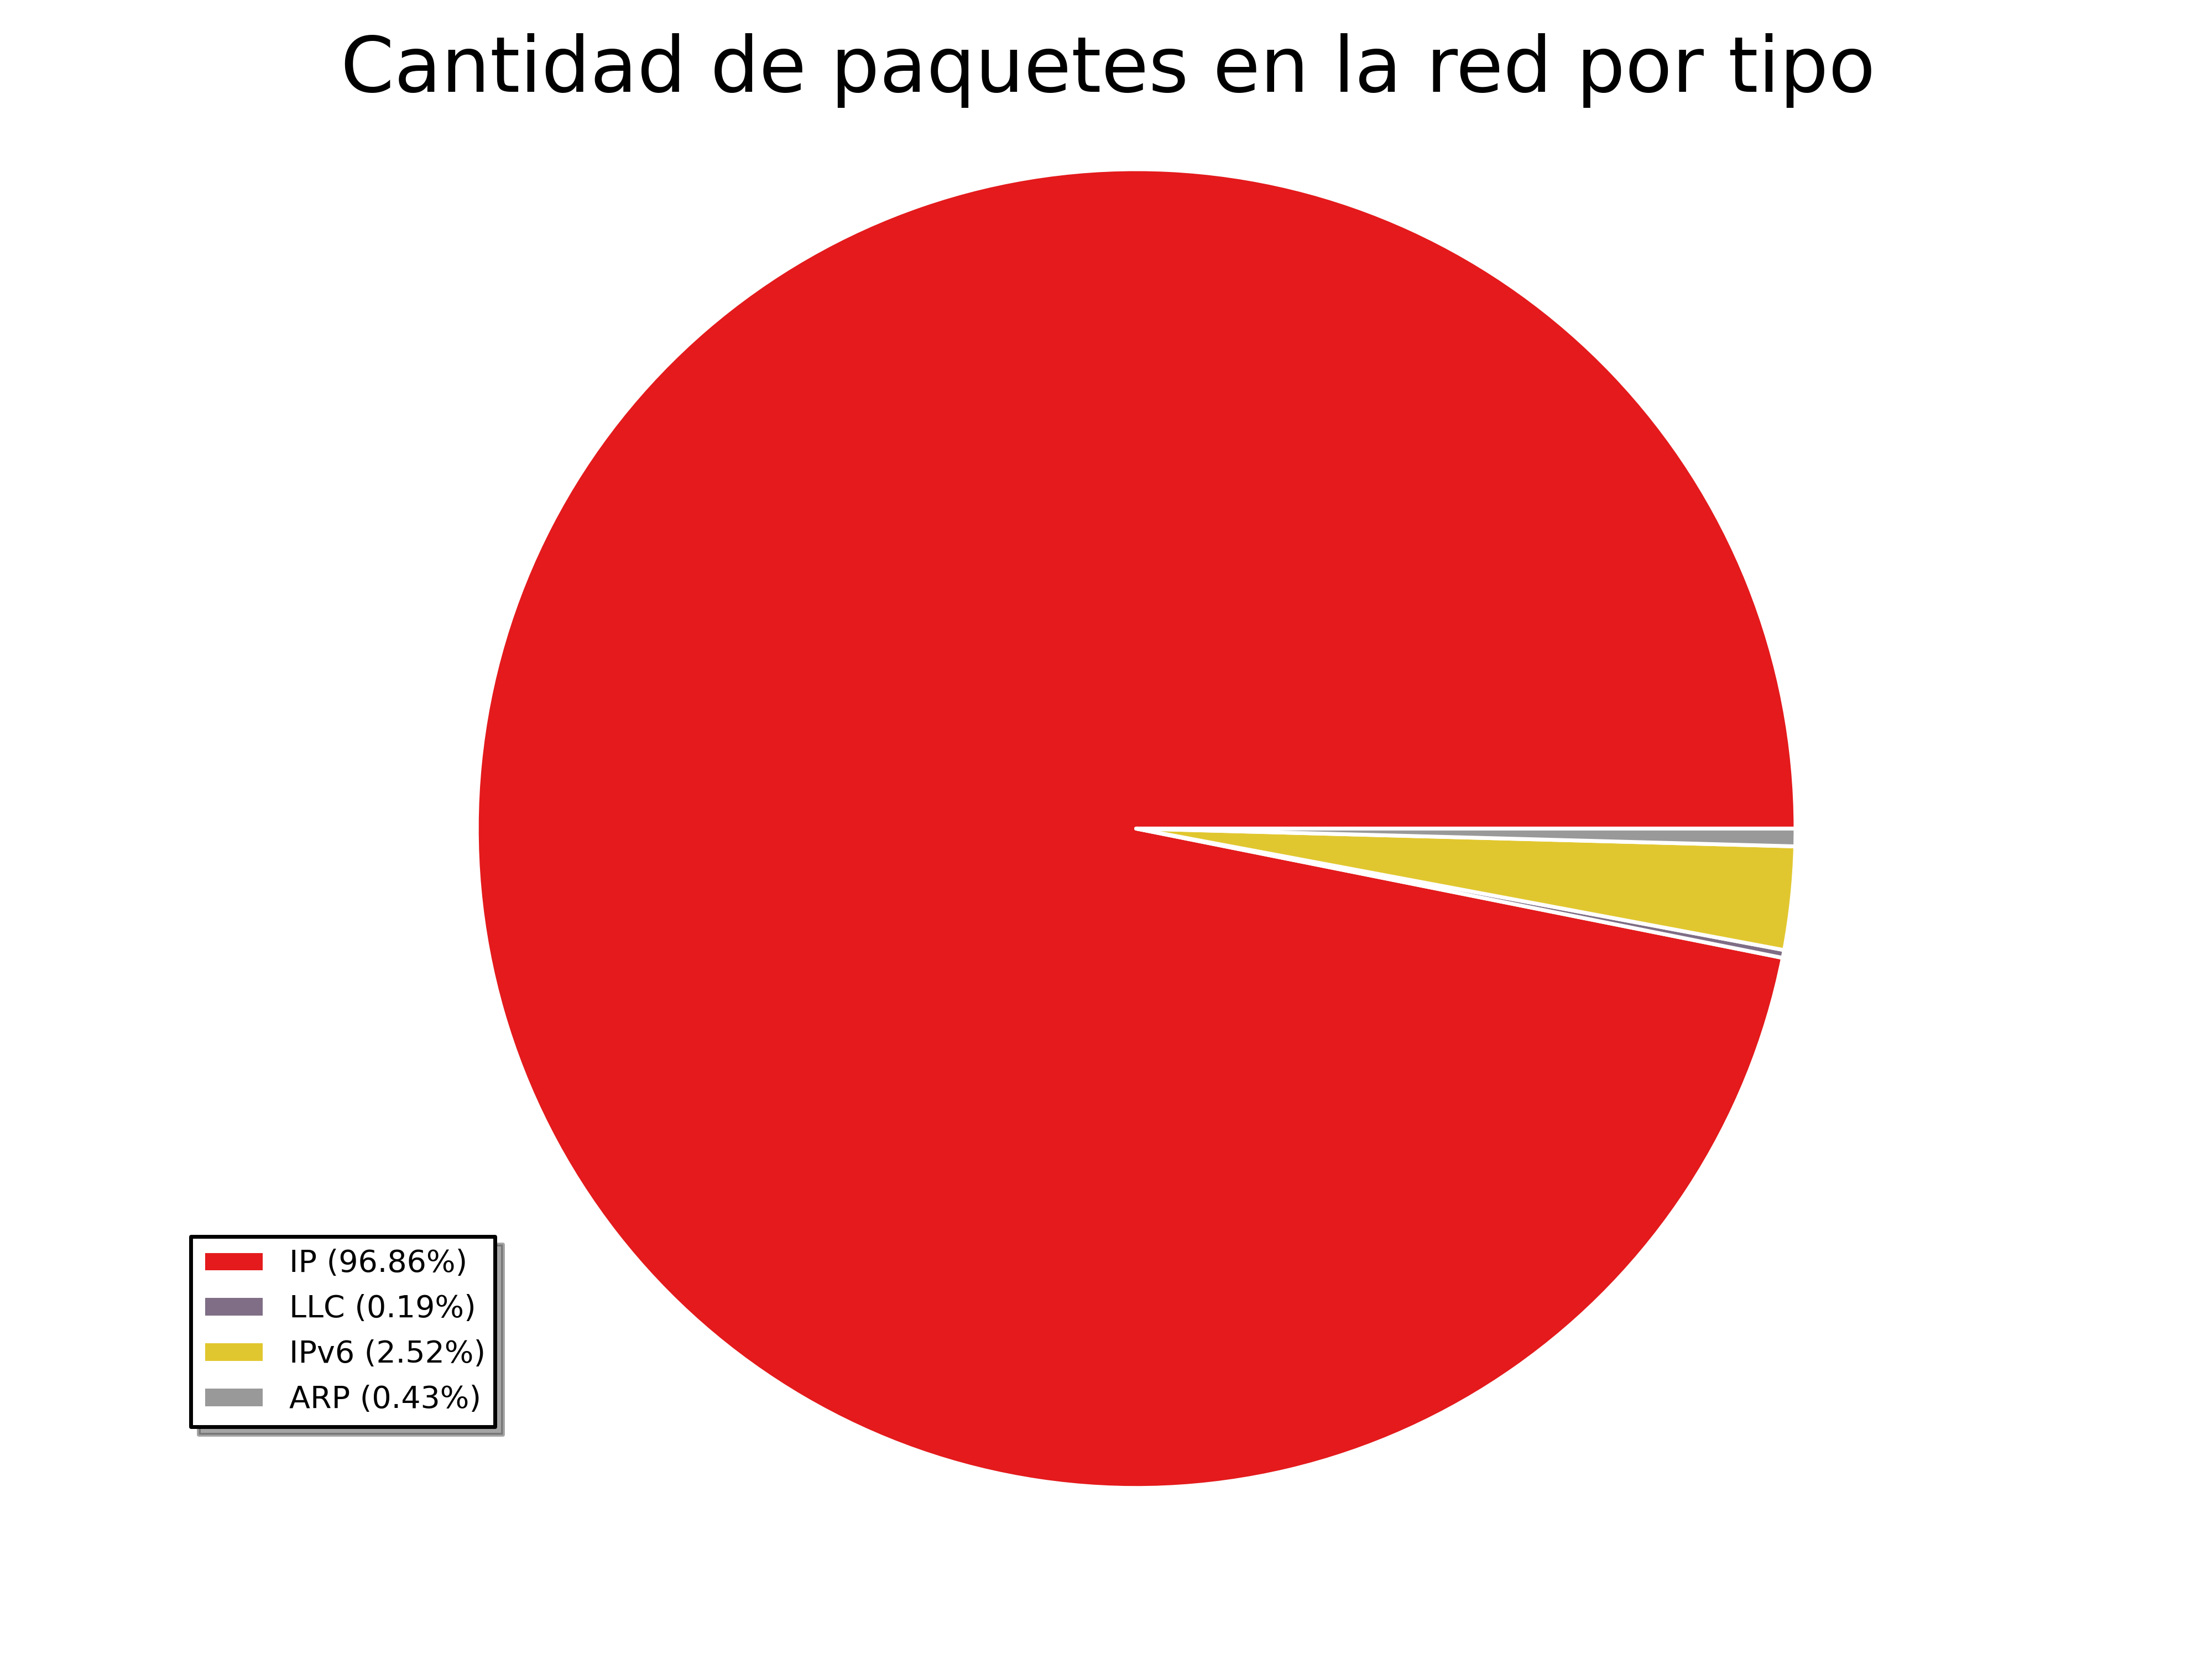
\includegraphics[width=\textwidth]{graficos/galerias_pacifico3_10min_pie_type.png}
    \caption{Fuente $S$}
    \label{fig:galerias_pacifico3_10min_pie_type}
  \end{minipage}
  \hfill
  \begin{minipage}[b]{0.48\textwidth}
    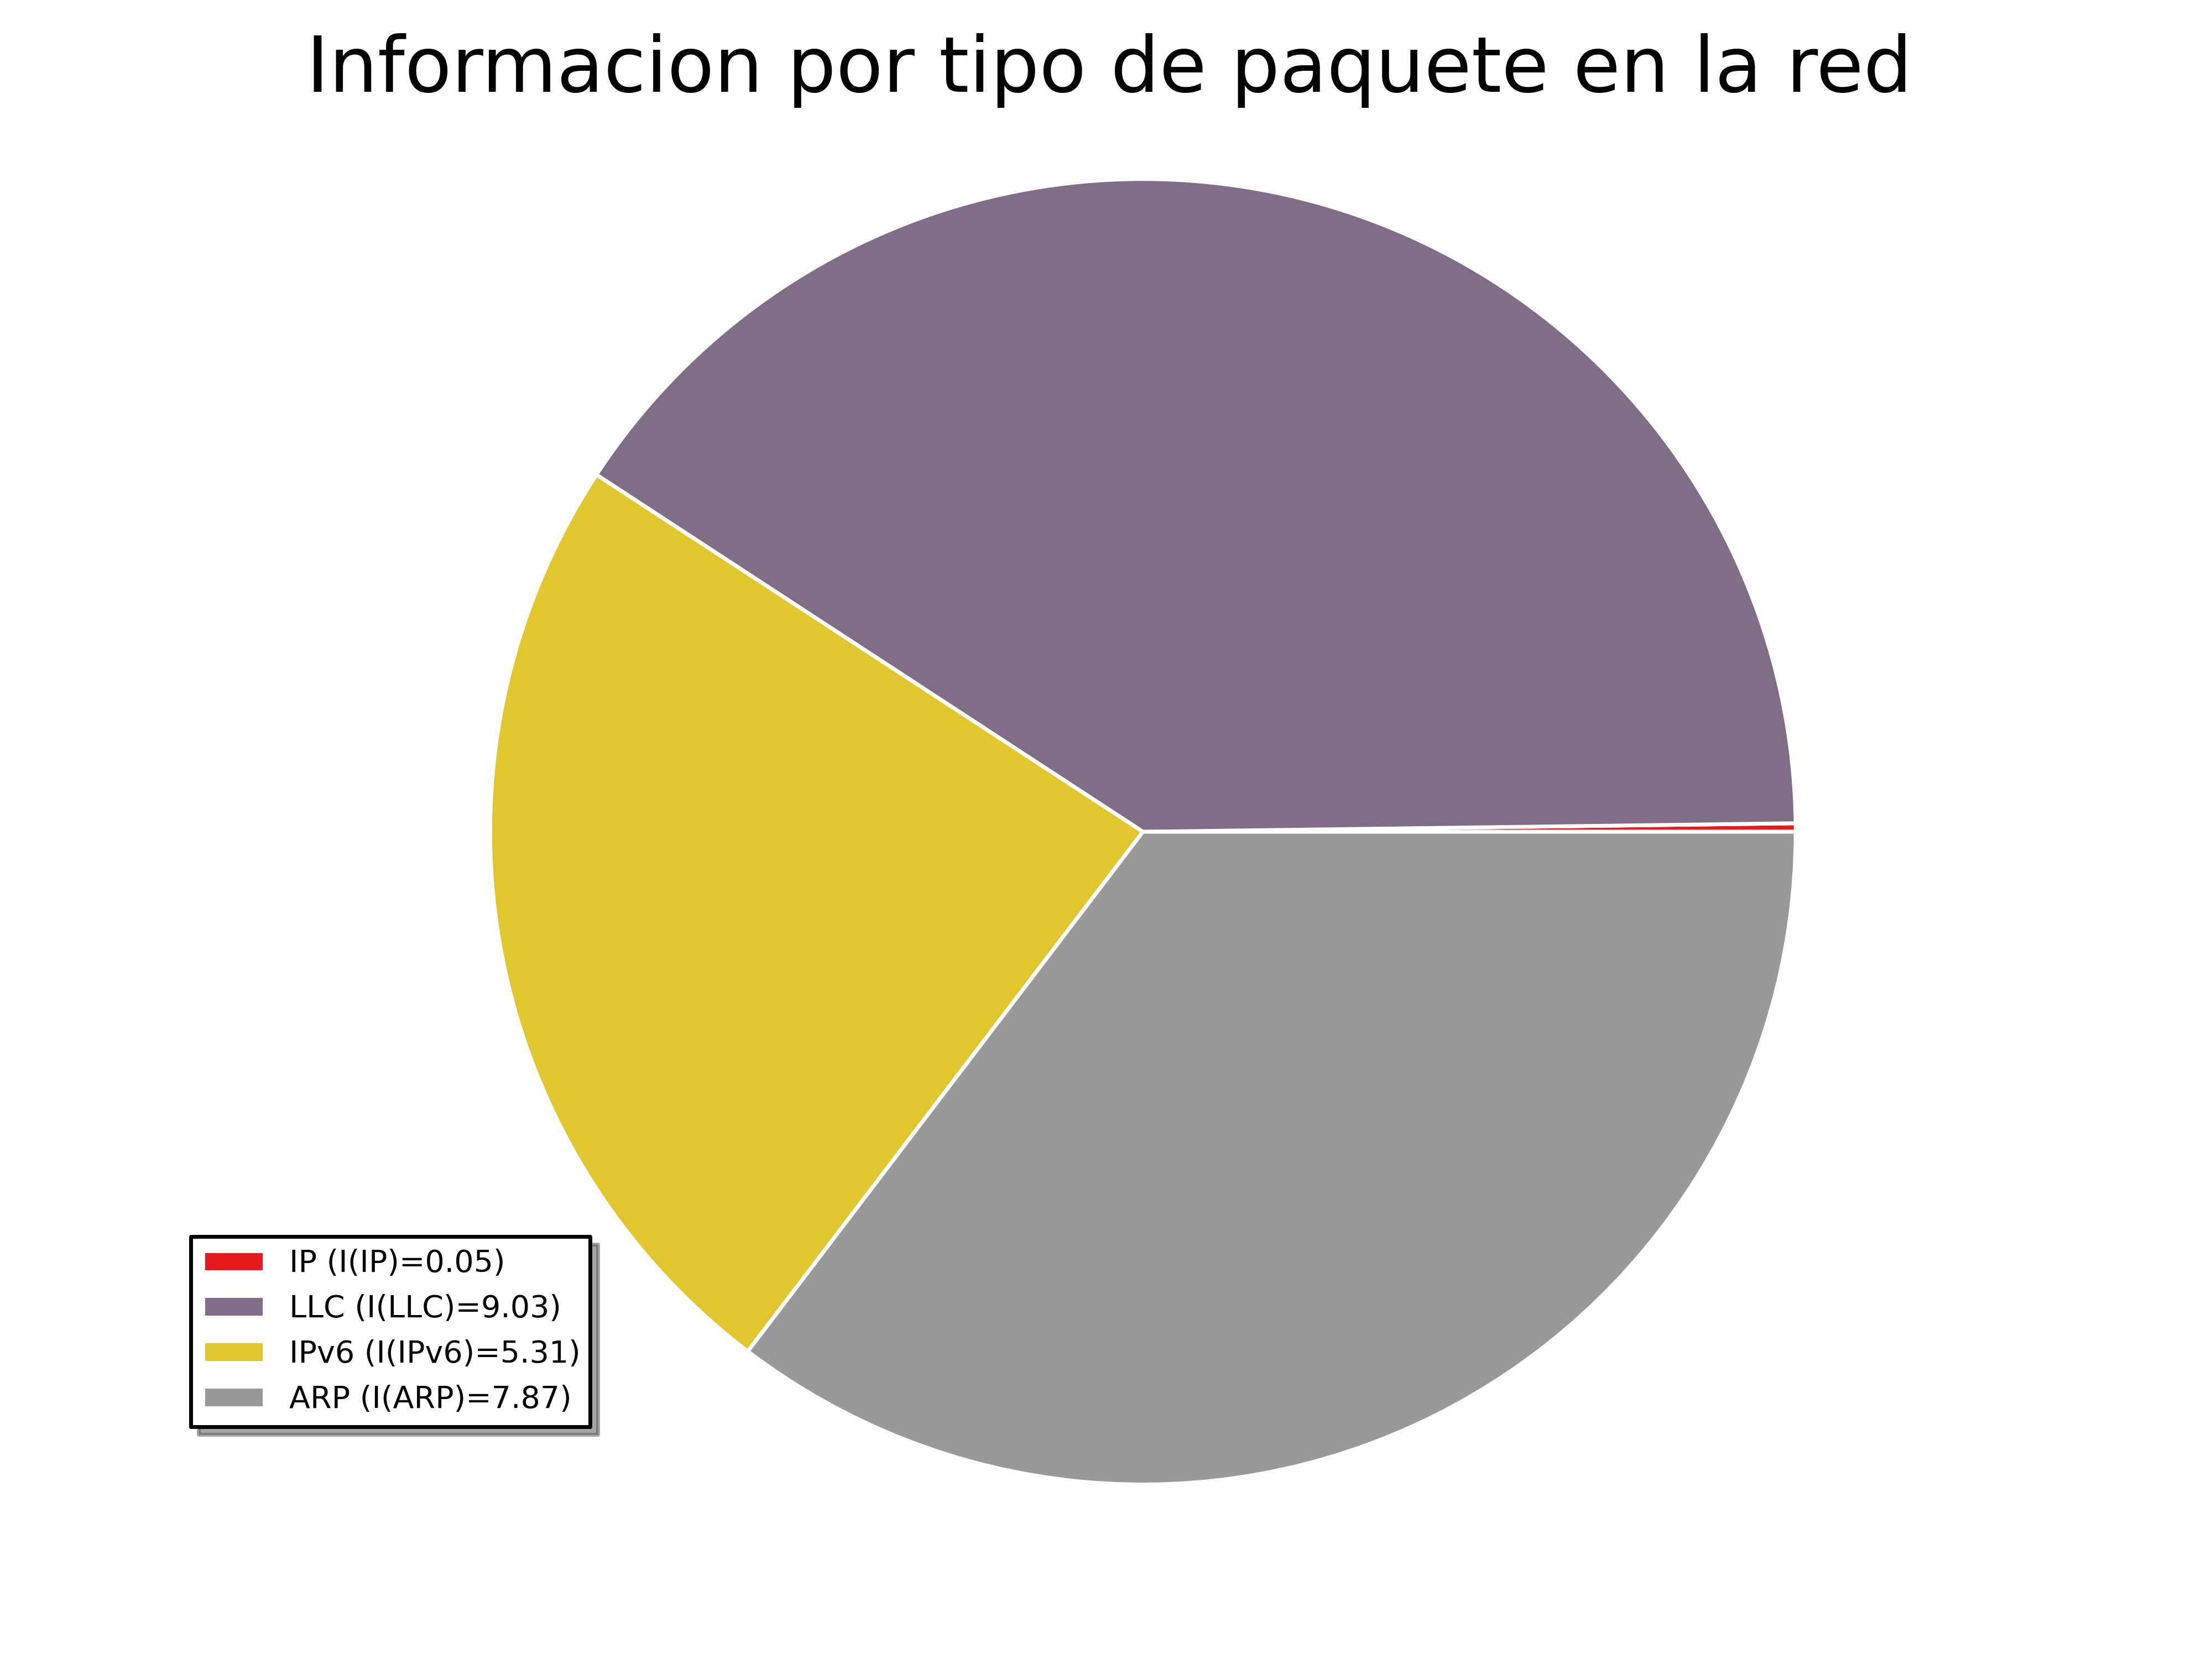
\includegraphics[width=\textwidth]{graficos/galerias_pacifico3_10min_pie_type_information.png}
    \caption{Fuente $S$}
    \label{fig:galerias_pacifico3_10min_pie_type_information}
  \end{minipage}
\end{figure}

En los gráficos Figura ~\ref{fig:galerias_pacifico3_10min_pie_type}. y Figura ~\ref{fig:galerias_pacifico3_10min_pie_type_information}. se puede observar que el protocolo IPV4 es el más frecuente y, por ende, el que brinda menos información.
\\
\\
\FloatBarrier

Mostramos ahora la frecuencia e información de cada IP en la red para la fuente $S_1$.

\begin{figure}[ht!]
  \centering
  \begin{minipage}[b]{0.48\textwidth}
    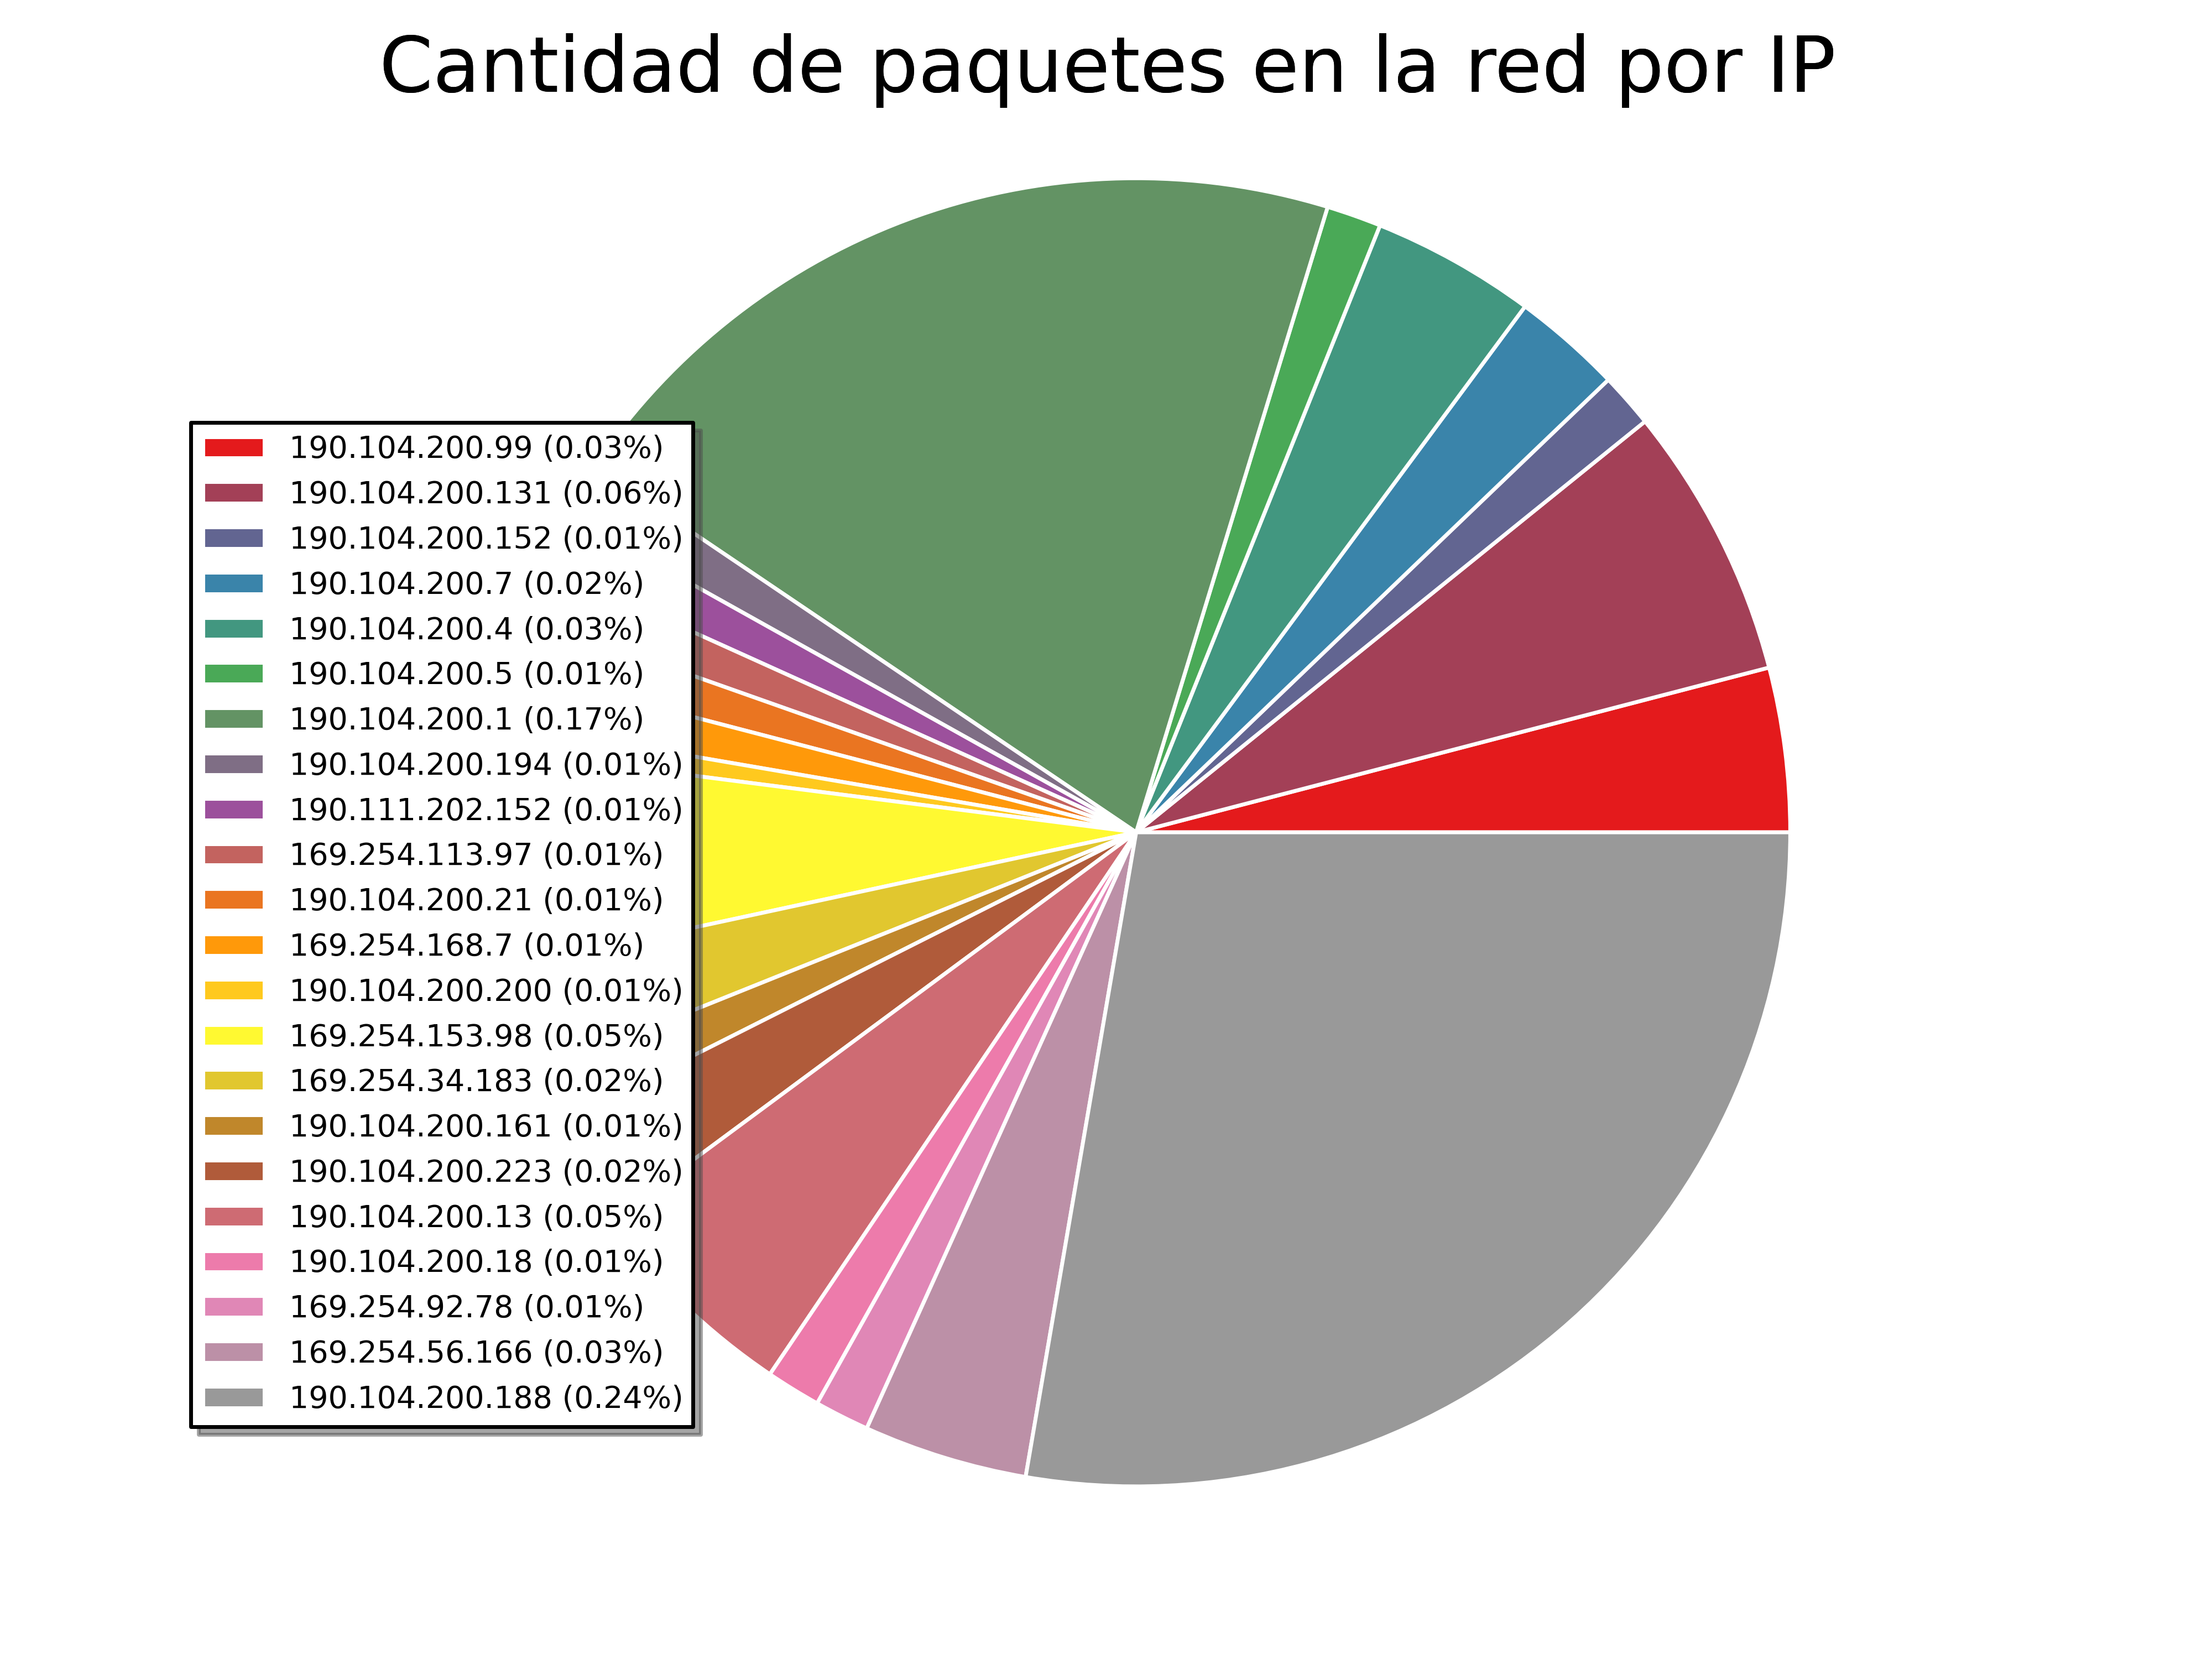
\includegraphics[width=\textwidth]{graficos/galerias_pacifico3_10min_pie_arp.png}
    \caption{Fuente $S_1$}
    \label{fig:galerias_pacifico3_10min_pie_arp}
  \end{minipage}
  \hfill
  \begin{minipage}[b]{0.48\textwidth}
    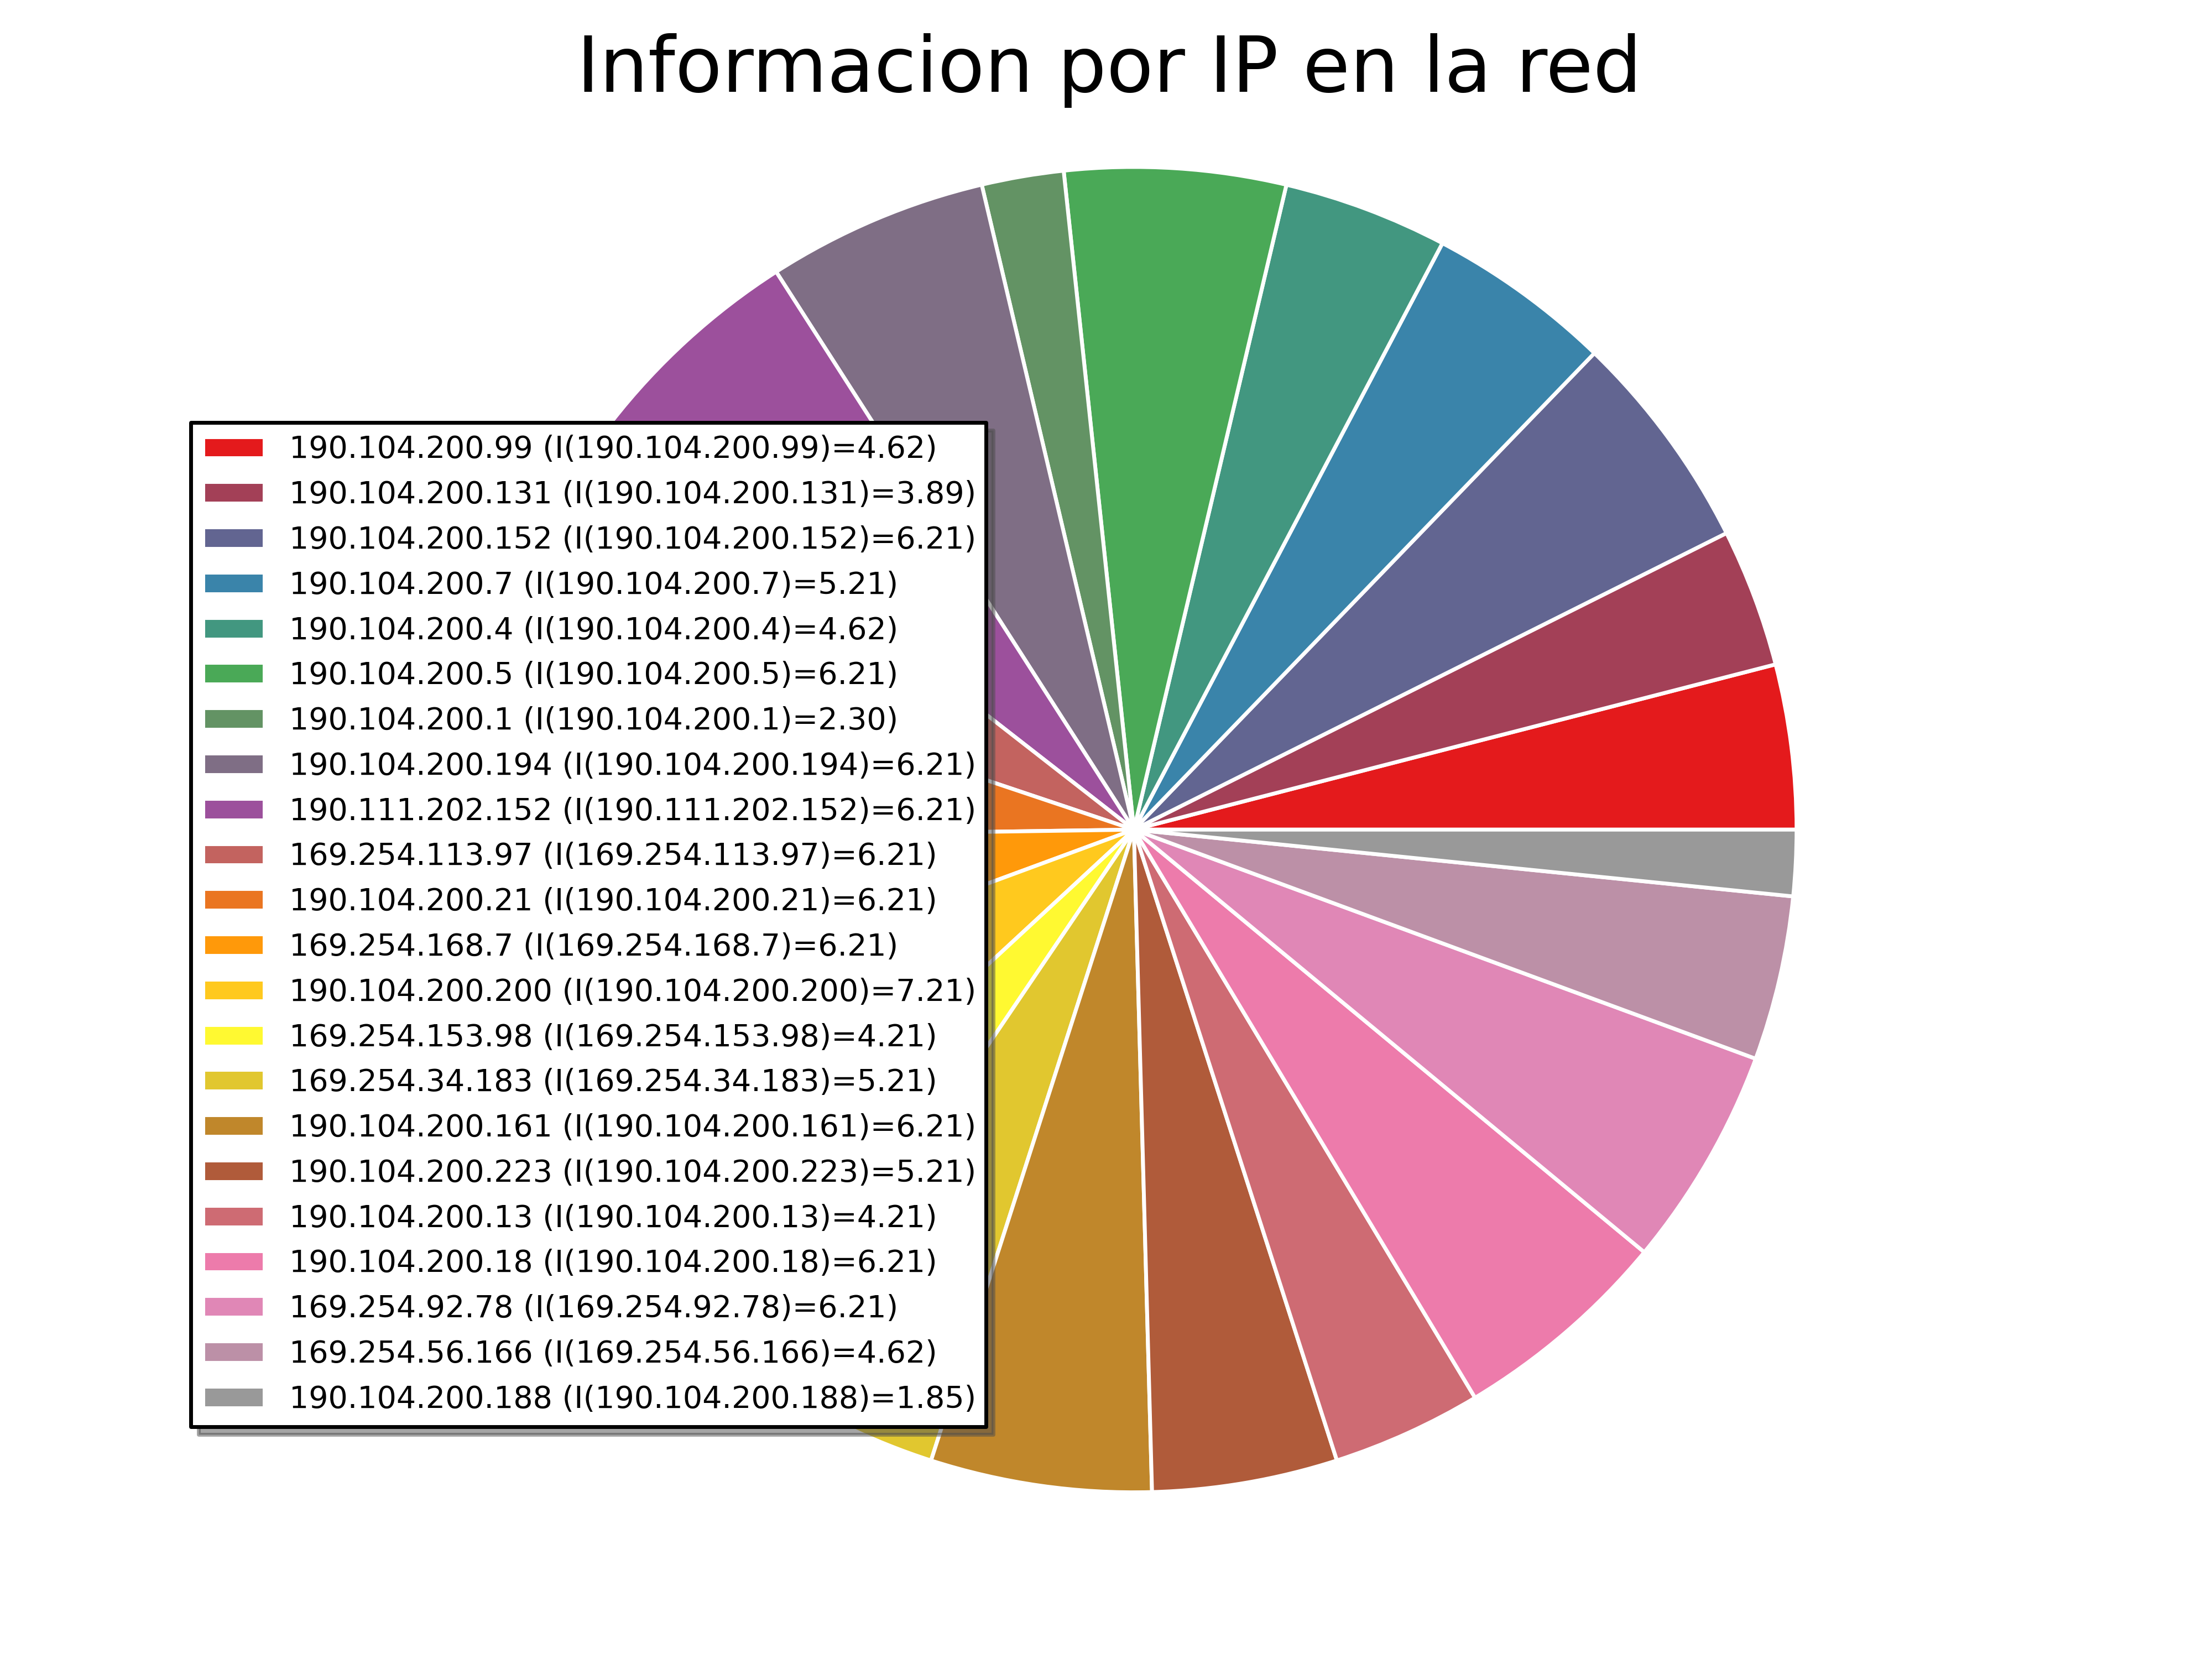
\includegraphics[width=\textwidth]{graficos/galerias_pacifico3_10min_pie_arp_information.png}
    \caption{Fuente $S_1$}
    \label{fig:galerias_pacifico3_10min_pie_arp_information}
  \end{minipage}
\end{figure}

En los gráficos Figura ~\ref{fig:galerias_pacifico3_10min_pie_arp}. y Figura ~\ref{fig:galerias_pacifico3_10min_pie_arp_information}.
podemos observar que las direcciones IP distinguidas son 192.104.200.5, 190.104.200.1 y 190.104.200.188. 

\FloatBarrier

\subsubsection{Nodos de la red}

En la Figura ~\ref{fig:galerias_pacifico3_10min_network} se muestra un grafo con los diferentes nodos en la red identificados por su dirección IP.

\begin{figure}[ht!]
  \centering
   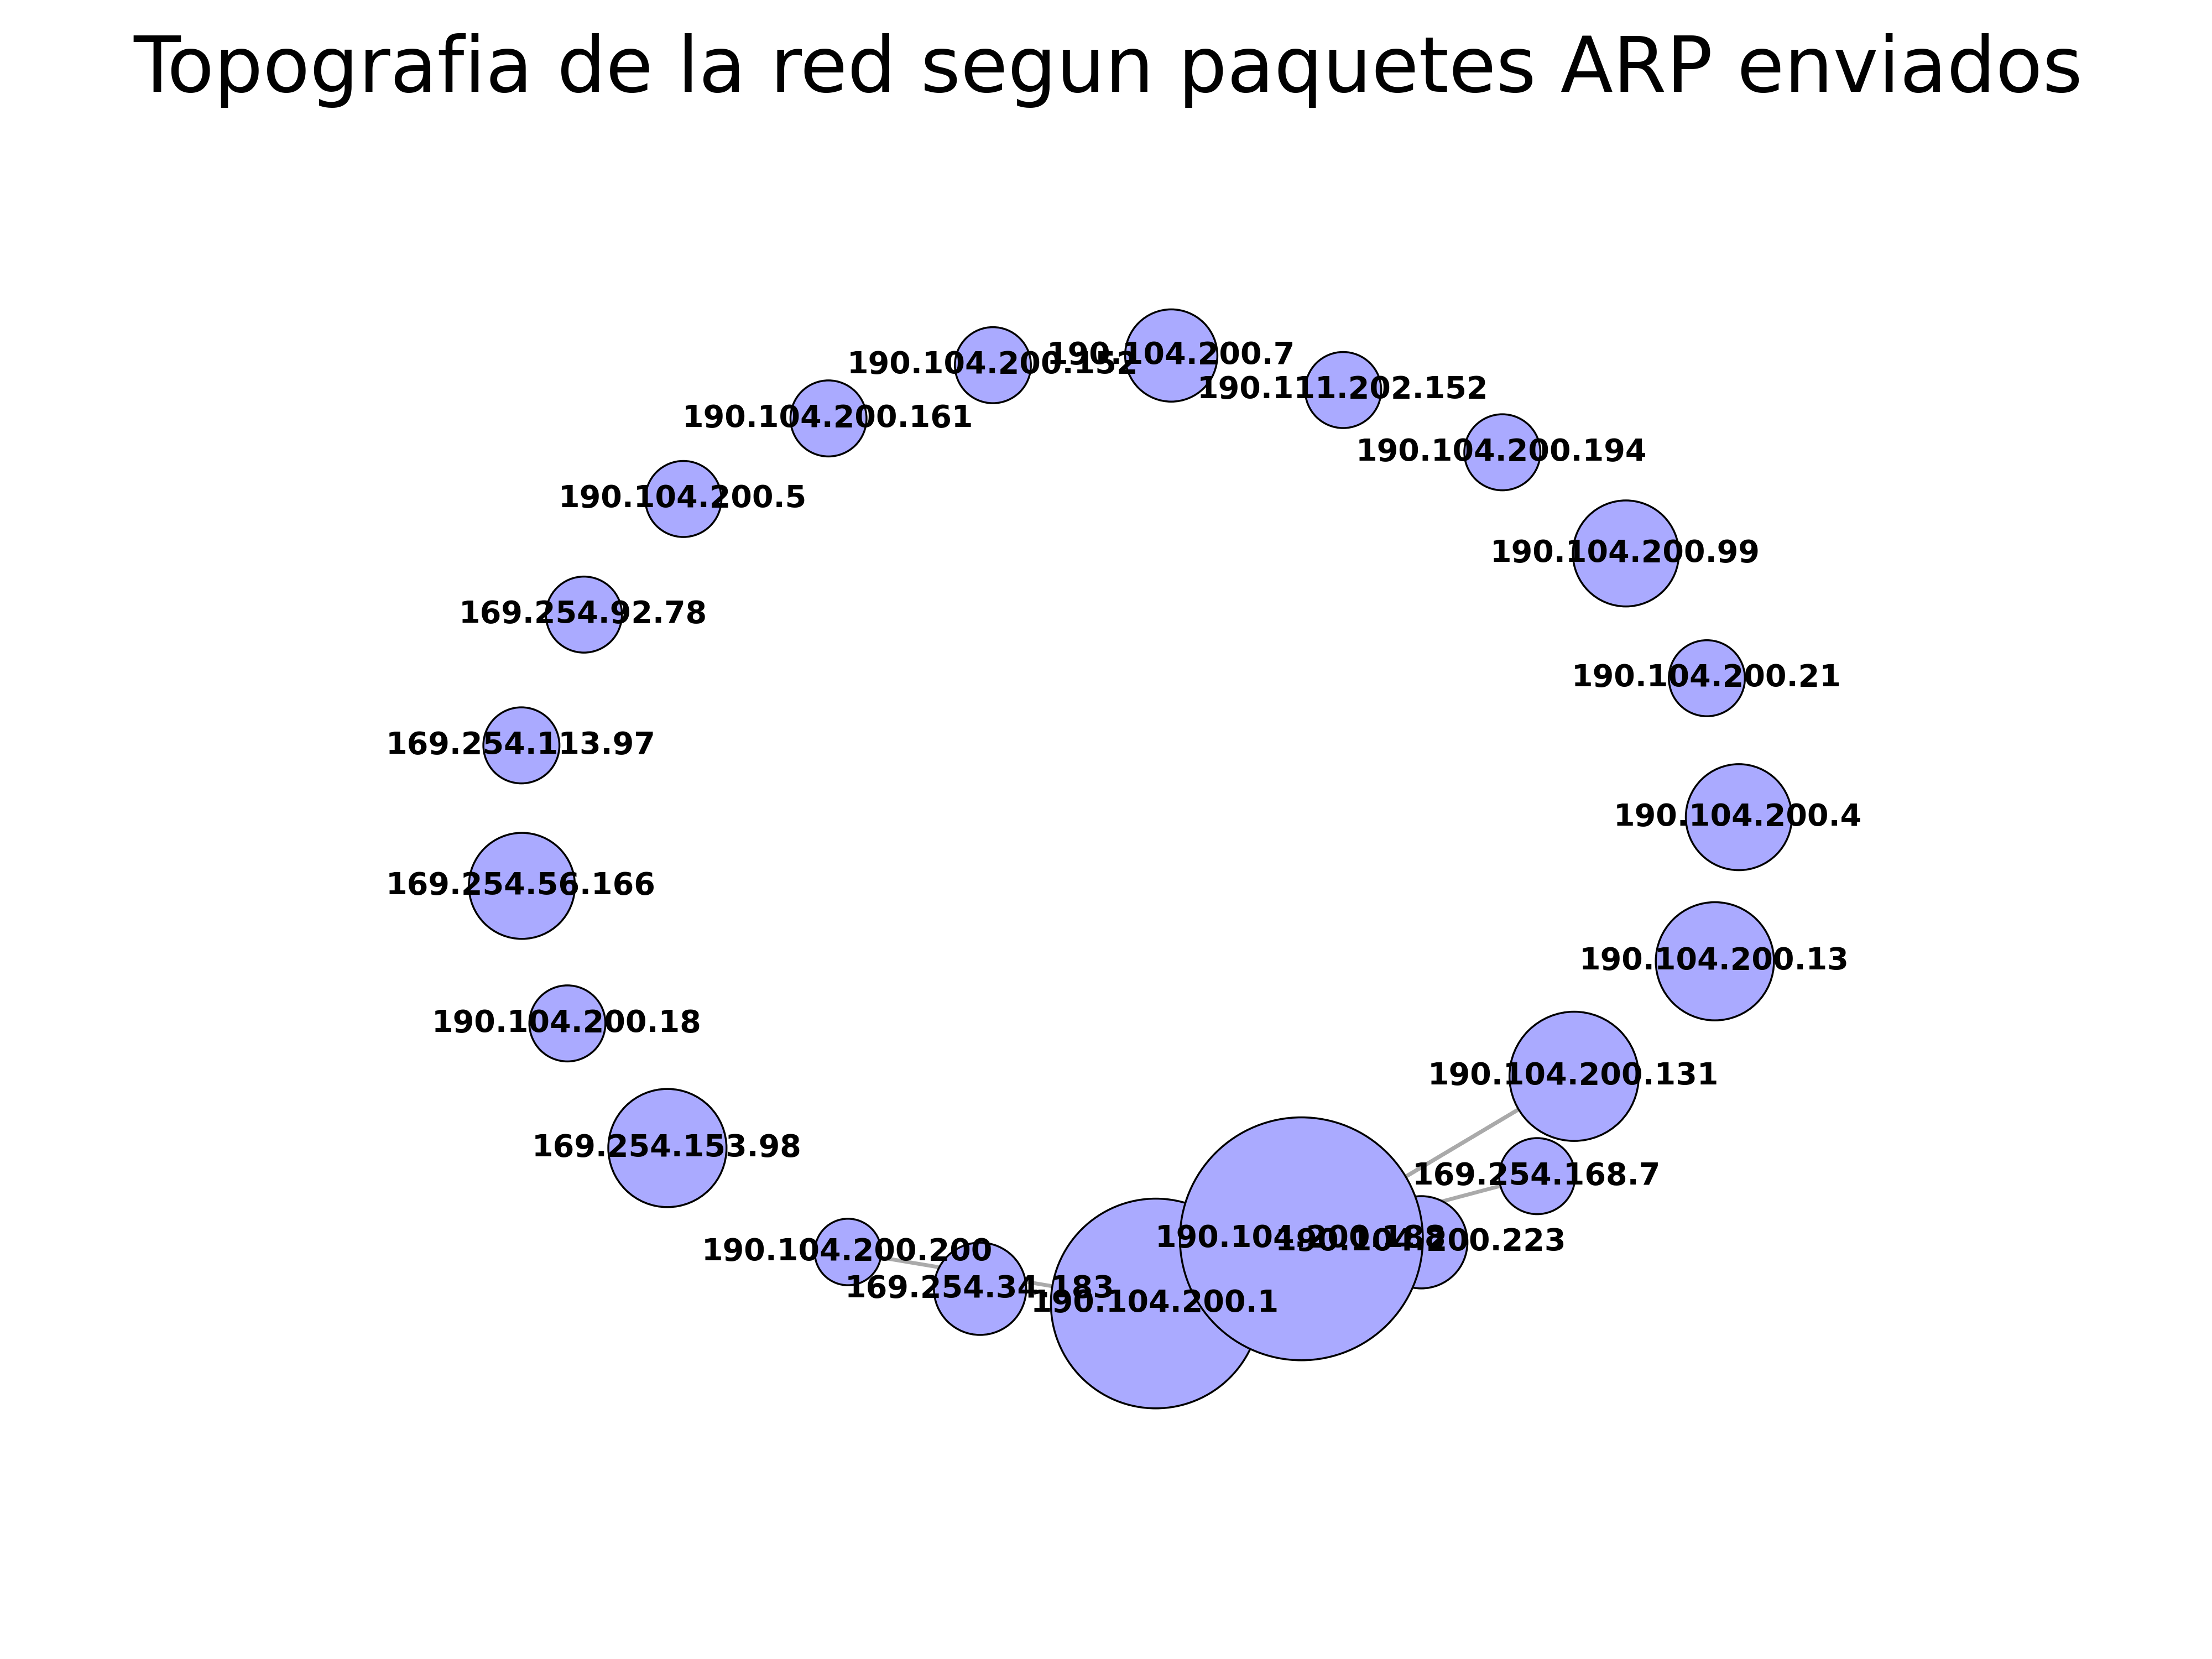
\includegraphics[width=0.7\textwidth]{graficos/galerias_pacifico3_10min_network.png}
  \caption{}
  \label{fig:galerias_pacifico3_10min_network}
\end{figure}

\FloatBarrier

\subsubsection{Análisis de la de entropía}

A continuación analizaremos histogramas con cortes en los valores de entropía, tanto para las IP de la red como para los tipos de protocolo.

\begin{figure}[ht!]
  \centering
  \begin{minipage}[b]{0.48\textwidth}
    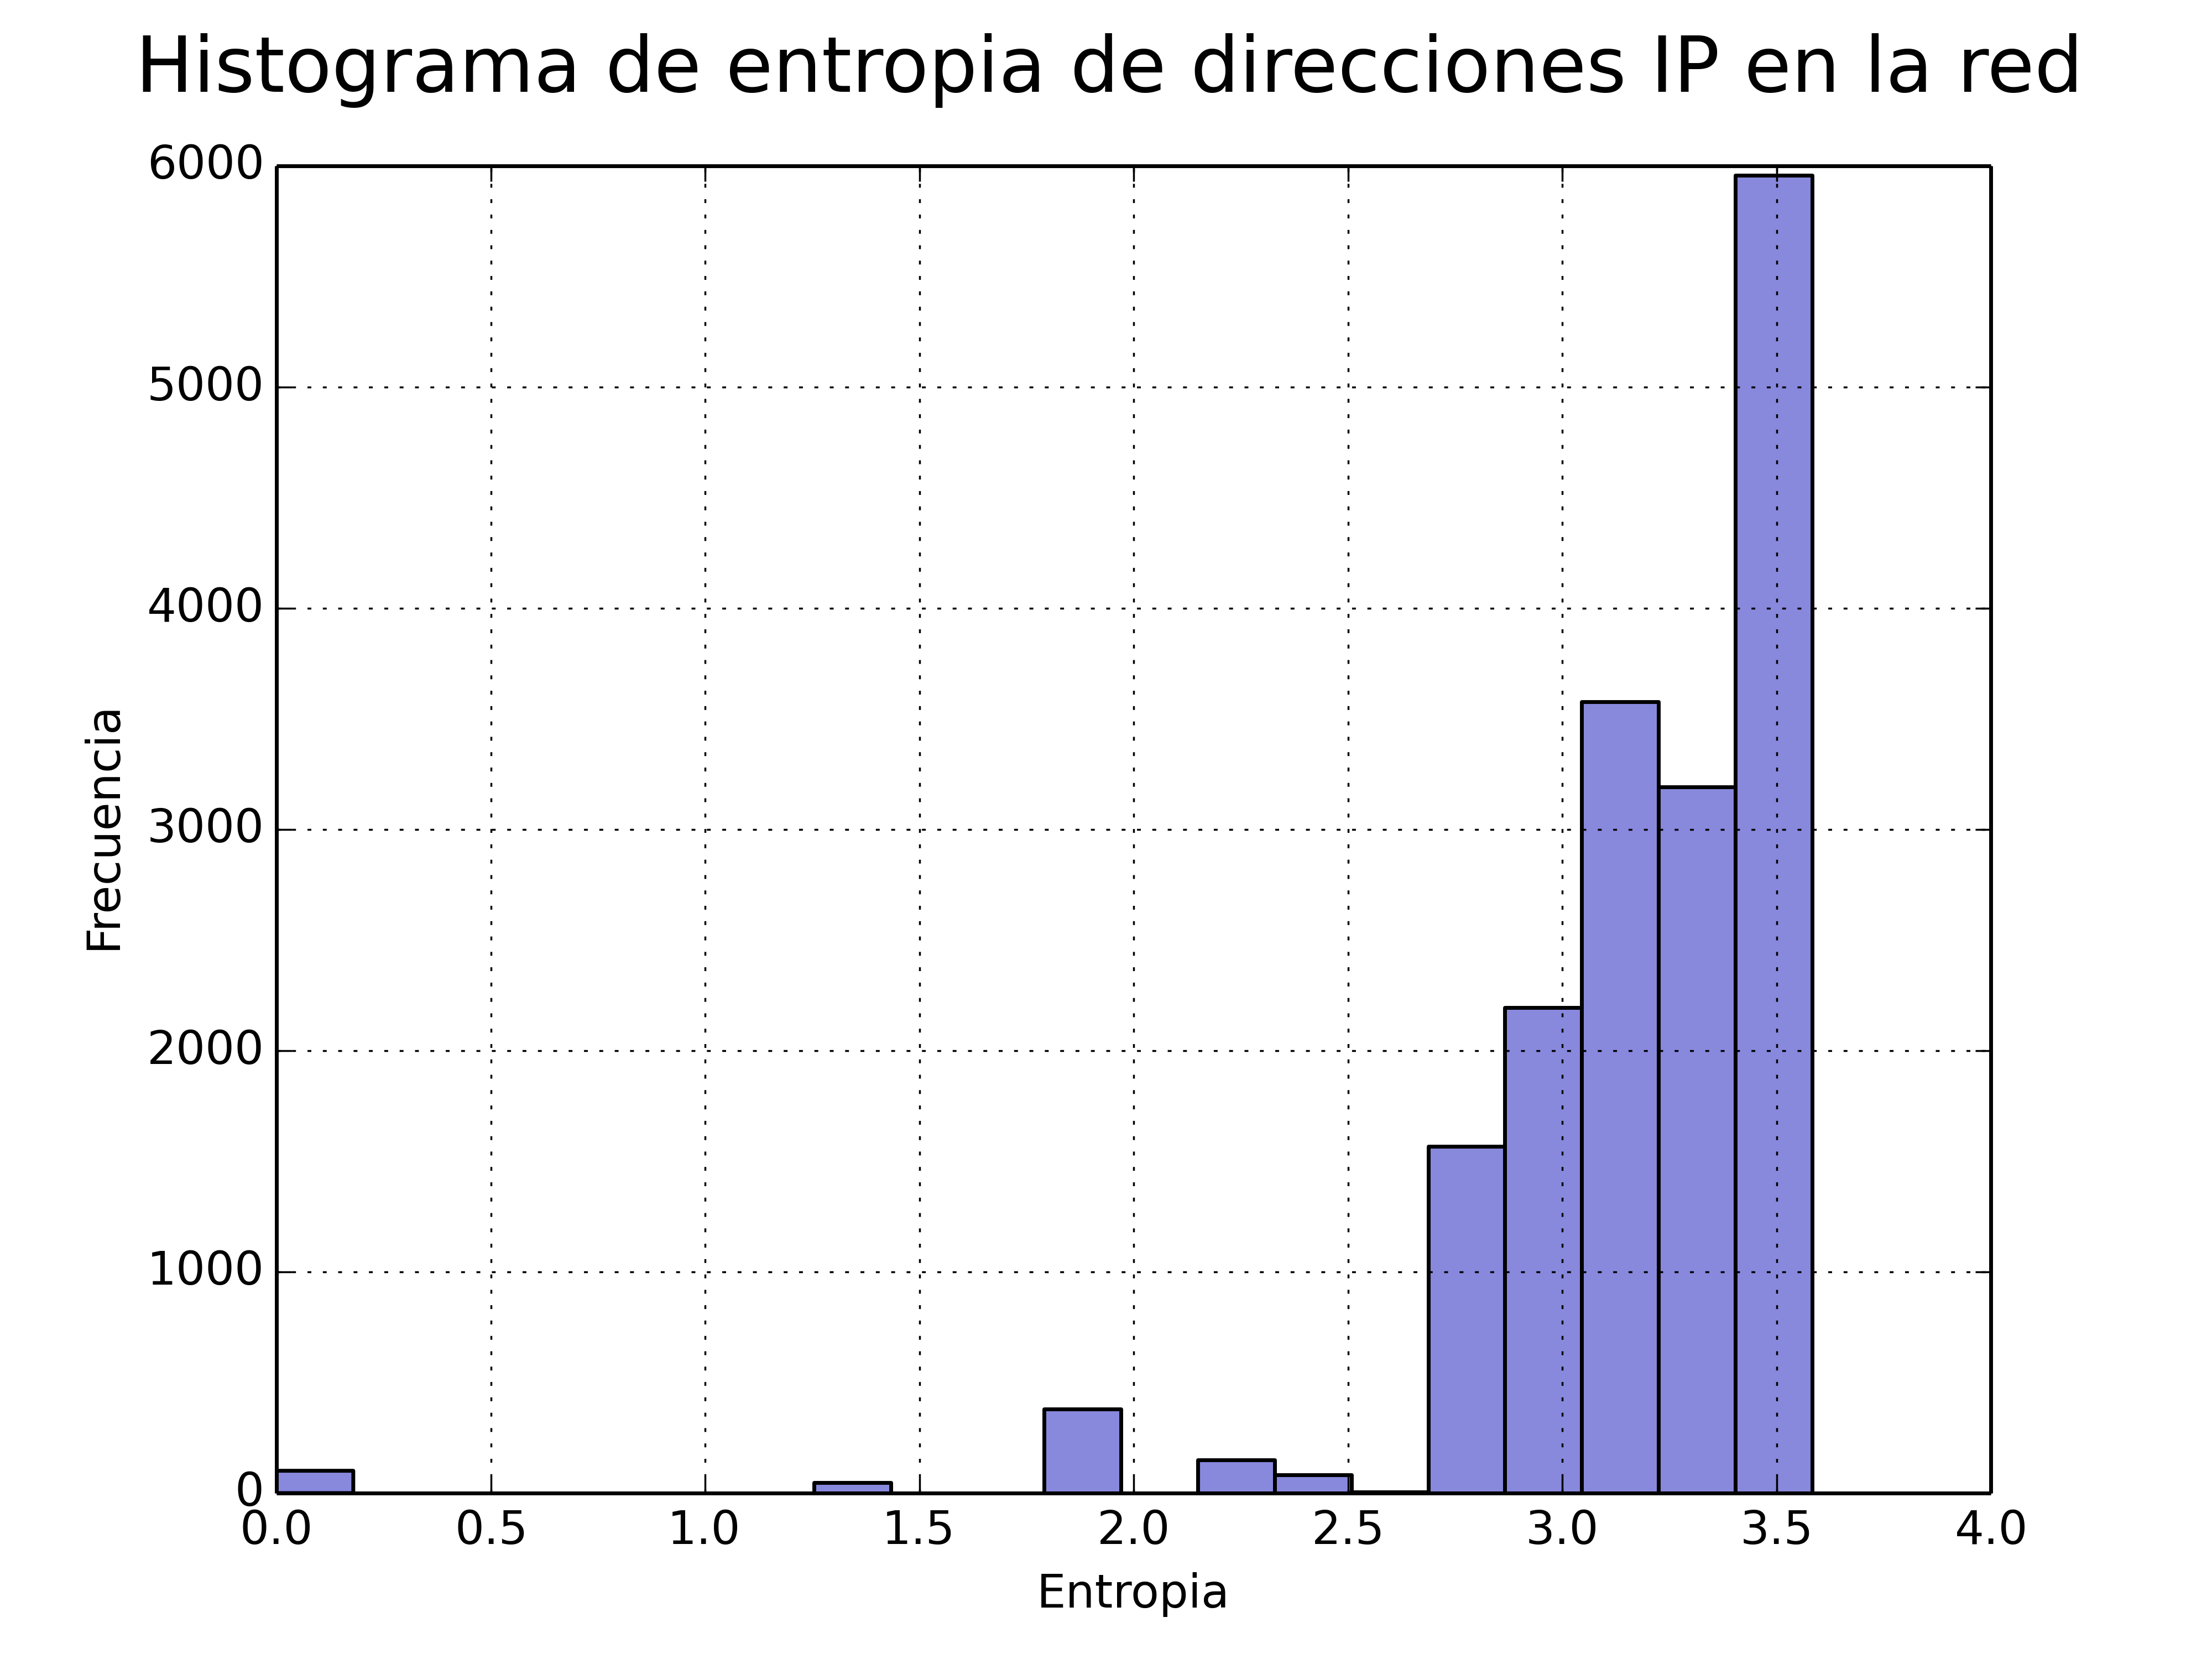
\includegraphics[width=\textwidth]{graficos/galerias_pacifico3_10min_hist_arp.png}
    \caption{Fuente $S$}
    \label{fig:galerias_pacifico3_10min_hist_arp}
  \end{minipage}
  \hfill
  \begin{minipage}[b]{0.48\textwidth}
    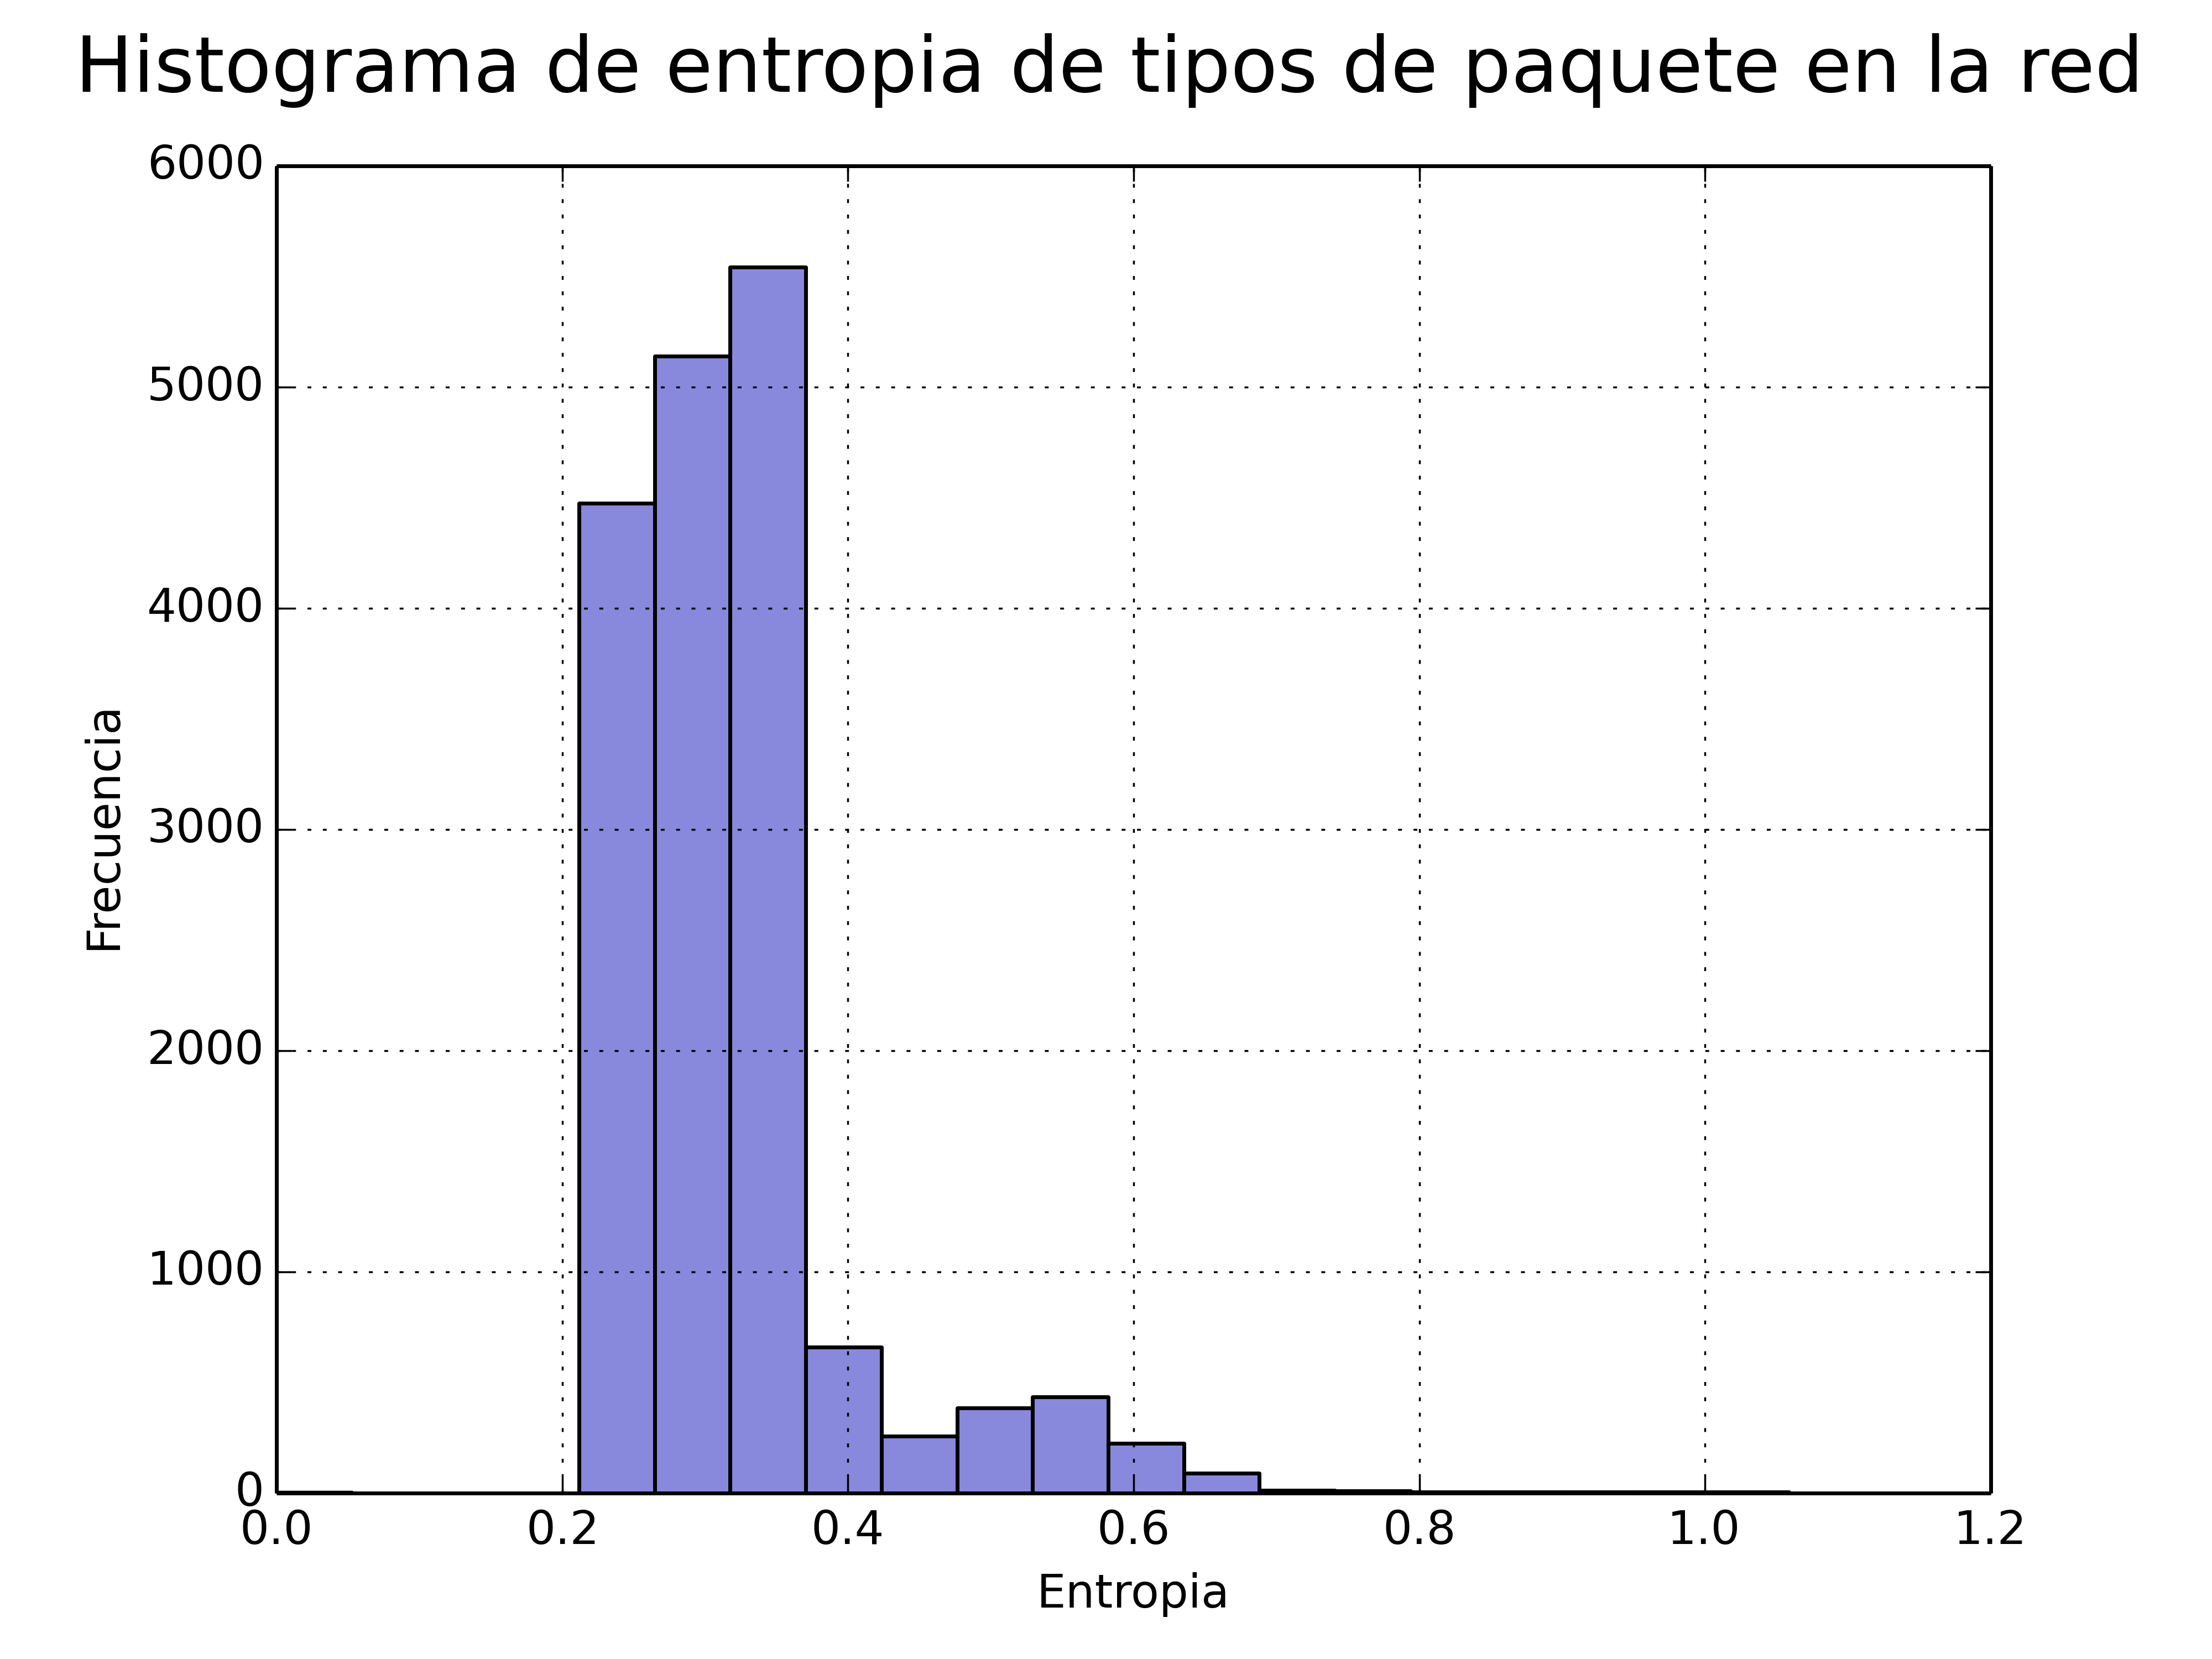
\includegraphics[width=\textwidth]{graficos/galerias_pacifico3_10min_hist_type.png}
    \caption{Fuente $S_1$}
    \label{fig:red_domestica_hist_arp}
  \end{minipage}
\end{figure}

Al igual que en las otras redes, podemos ver que la entropía en la fuente $S$ es menor que en la fuente $S_1$, debido a que en la primera, los símbolos son más predecibles.